\section{Introducción y Teoria}
\subsection{Aprendizaje Hebbiano}

El aprendizaje Hebbiano consiste basicamente en el ajuste de los pesos de las conexiones, de acuerdo con la correlacion de los valores de activacion (salidas) de las neuronas conectadas.

El aprendizaje implica que el elemento de proceso cambia su comportamiento de entrada/salida en respuesta a un entorno. La salida se calcula como el resultado de una función de transferencia de la entrada ponderada.

El peso entre dos neuronas se incrementa si las dos neuronas se activan simultáneamente y se reduce si se activan por separado. Los nodos que tienden a ser positivos o negativos al mismo tiempo tienen fuertes pesos positivos, mientras que aquellos que tienden a ser contrarios tienen fuertes pesos negativos.

La siguiente es una formulación matemática del aprendizaje hebbiano:

$w_{ij} = x_i x_j$

donde $w_{ij}$ es el peso de la conexión de la neurona j a la neurona i y $x_{i}$ el valor de entrada para la neurona i. Hay que tener en cuenta que este es el modelo de aprendizaje (pesos actualizados después de cada ejemplo de entrenamiento). En otras redes las conexiones $w_{ij}$ se ponen a cero si  i=j  (no se permiten conexiones reflexivas). Con neuronas binarias (valores de activación de 0 ó 1) las conexiones se establecen a 1 si las neuronas conectadas tienen el mismo patrón de activación.

La regla de Hebb se generaliza frecuentemente como:

\begin{center}
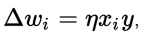
\includegraphics[width=0.15\textwidth]{img/formula1}
\end{center}

o el cambio en el peso $w_{i}$ de la sinapsis número i es igual a la tasa de aprendizaje $\eta$   por la entrada número i $x_{i}$ por la respuesta postsináptica  y. A menudo se cita el caso de una neurona lineal,

\begin{center}
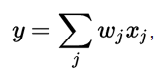
\includegraphics[width=0.15\textwidth]{img/formula2}
\end{center}


\subsection{Aprendizaje Competitivo}


En el aprendizaje competitivo las neuronas compiten unas con otras con el fin de llevar a cabo una tarea dada. Se pretende que cuando se presente a la red un patrón de entrada, sólo una de las neuronas de salida (o un grupo de vecinas) se active.

Por tanto, las neuronas compiten por activarse, quedando finalmente una como neurona vencedora y anuladas el resto, que son forzadas a sus valores de respuesta mínimos.

El objetivo de este aprendizaje es categorizar los datos que se introducen en la red. Se clasifican valores similares en la misma categoría y, por tanto, deben activar la misma neurona de salida

Las clases o categorías deben ser creadas por la propia red, puesto que se trata de un aprendizaje no supervisado, a través de las correlaciones entre los datos de entrada.

\newpage
\subsubsection{Los mapas auto-organizados de Kohonen (SOM)}

Un modelo SOM está compuesto por dos capas de neuronas. La capa de entrada (formada por N neuronas, una por cada variable de entrada) se encarga de recibir y transmitir a la capa de salida la información procedente del exterior. La capa de salida (formada por M neuronas) es la encargada de procesar la información y formar el mapa de rasgos.

Normalmente, las neuronas de la capa de salida se organizan en forma de mapa bidimensional como se muestra en la figura:

\begin{center}
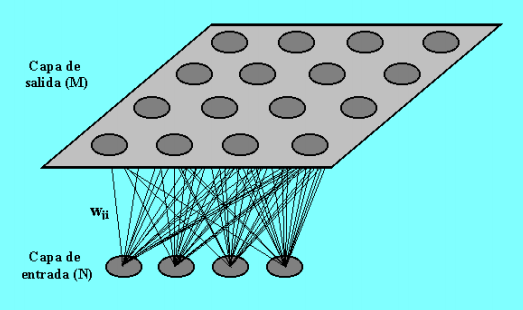
\includegraphics[width=0.5\textwidth]{img/neuronas1}
\end{center}


Las conexiones entre las dos capas que forman la red son siempre hacia delante, es decir, la información se propaga desde la capa de entrada hacia la capa de salida. Cada neurona de entrada i está conectada con cada una de las neuronas de salida j mediante un peso $w_{ji}$. De esta forma, las neuronas de salida tienen asociado un vector de pesos $W_j$ llamado vector de referencia, debido a que constituye el vector prototipo (o promedio) de la categoría representada por la neurona de salida j. Así, el SOM define una proyección desde un espacio de datos en alta dimensión a un mapa bidimensional de neuronas.

Entre las neuronas de la capa de salida, puede decirse que existen conexiones laterales de excitación e inhibición implícitas, pues aunque no estén conectadas, cada una de estas neuronas va a tener cierta influencia sobre sus vecinas. Esto se consigue a través de un proceso de competición entre las neuronas y de la aplicación de una función denominada de vecindad , que produce la topología o estructura del mapa. Las topologías más frecuentes son la rectangular y la hexagonal.
Las neuronas adyacentes pertenecen a una vecindad Nj de la neurona j. La topología y el número de neuronas permanece fijo desde el principio. El número de neuronas determina la suavidad de la proyección, lo cual influye en el ajuste y capacidad de generalización del SOM.	

Durante la fase de entrenamiento, el SOM forma una red elástica que se pliega dentro de la nube de datos originales. El algoritmo controla la red de modo que tiende a aproximar la densidad de los datos. Los vectores de referencia del codebook se acercan a las áreas donde la densidad de datos es alta. 

Eventualmente unos pocos vectores el codebook están en áreas donde existe baja densidad de datos.

Un ejemplo de como quedarian las agrupaciones: 

\begin{center}
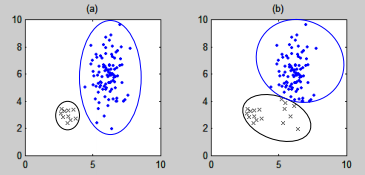
\includegraphics[width=0.5\textwidth]{img/agrupaciones1}
\end{center}